\subsection{Модифицированные нечеткие числа}

В~статье~\cite{Lebedev}, для преодоления изложенных в предыдущем параграфе недостатков нечётких алгебр, для решения нечётких задач был предложен следующий подход. Исходная задача $\tilde{Y}=f\left( {\tilde{X}} \right)$ с нечёткими числовыми параметрами рассматривается как совокупность задач с интервальной неопределенностью
\begin{equation}
\label{eq:alpha-equivalence}
	\tilde{Y} = f\left( \tilde X \right)\to \bigcup\limits_{\alpha =0}^{1}{y_\alpha}=f\left( X_\alpha \right)
\end{equation}
с последующим переходом к полной определённости. Для этого на каждом $\alpha$-уровне внутри интервала $X_\alpha$ выбирается точка $\bar{x}\left( \alpha  \right)$. В~\cite{Lebedev} для этого используется средняя точка $\alpha$-интервала
\begin{equation}
  \label{eq:L-transform-midpoint}
  \overline{x}\left( \alpha  \right)=\frac{x^L\left( \alpha  \right)+x^R\left( \alpha  \right)}{2}
\end{equation}

Для треугольных чисел $\bar{x}\left( \alpha  \right)$ является линейной функцией ввиду линейности $x^L\left( \alpha  \right)$ и $x^R\left( \alpha  \right)$. После решения $N$~чётких $\alpha $-уровневых задач полученные результаты $y\left( \alpha  \right)$ аппроксимируются нечётким числом
\begin{equation*}
  \tilde Y^{*}=\left\{ y(\alpha )\left| \mu_{\tilde Y}(y)=\alpha \right. \right\}
\end{equation*}
которое называется модифицированным решением задачи $\tilde{Y}=f\left( \tilde X \right)$. В~статье утверждается, что в реальных задачах модифицированного решения достаточно для, например, поддержки принятия решений. 

Предлагаемый подход в своей основе имеет факторизацию, т.\,е.~декомпозицию нечётких чисел по~$\alpha$-уровням, однако в~\cite{Lebedev} рассмотрен только частный случай выбора точки внутри интервала, а также отсутствует строгое математическое доказательство применимости метода, предложенное позднее в~\cite{Vorontsov_PI}.

Если рассмотреть данный подход с точки зрения нечётких алгебр, то решение задачи с~использованием факторизации нечётких чисел представляется как переход от использования алгебр <<полноценных>> нечётких чисел к~алгебрам для~чисел $LL/RR$-типа. Действительно, функция принадлежности LL/RR-числа является обратной к~функции, которая определяет точки $\bar{x}\left(\alpha \right)$:
\begin{equation}
\label{eq:modified-inverse-function}
  \mu_{\tilde A^{*}}\left( x \right)={\left( \bar{x}\left( \alpha  \right) \right)}^{-1}
\end{equation}

\begin{mydef}
Число $\tilde A^{*}$, получаемое из числа $\tilde{A}$ с помощью преобразования~\eqref{eq:modified-inverse-function}, будем называть модифицированным нечётким числом.
\end{mydef}
Модифицированное нечёткое число является числом $LL/RR$-типа, поскольку один из коэффициентов нечёткости равен нулю, а функция принадлежности имеет только левую или правую ветвь. В дальнейшем для модифицированных чисел, наряду с обозначением $\tilde A^{*}$, будем использовать обозначение $\bar{x}\left( \alpha  \right)$, которое указывает на механизм их построения как совокупности точек на выбранных $\alpha $-интервалах.

\textbf{Пример.} Пусть $\tilde{A}=\left\langle 2;2;4 \right\rangle $. Найдём модифицированное число $\tilde A^{*}$ в соответствие с~\eqref{eq:L-transform-midpoint}.
Вначале запишем функцию принадлежности числа $\tilde A^{*}$:
\begin{equation*}
	\mu_{\tilde A} \left( x \right)=\left\{ 
	  \begin{aligned}
        & \frac{x}{2};\ 0\le x\le 2 \\ 
        & \frac{6-x}{4};\ 2<x\le 6 \\ 
        & 0;\ x<0\ \ x>6 \\ 
      \end{aligned} \right.
\end{equation*}

Используя выражения~\eqref{eq:membership-abm-form}, получим
\begin{equation*}
	\left[ \begin{aligned}
      & {{x}^{L}}\left( \alpha  \right)=m-a+a\alpha =2-2+2\alpha =2\alpha  \\ 
      & {{x}^{R}}\left( \alpha  \right)=m+b-b\alpha =2+4-4\alpha =6-4\alpha  \\ 
    \end{aligned} \right.
\end{equation*}

Тогда, согласно~\eqref{eq:L-transform-midpoint}, получим:
\begin{equation*}
	\bar{x}\left( \alpha  \right)=\frac{{{x}^{L}}\left( \alpha  \right)+{{x}^{R}}\left( \alpha  \right)}{2}=\frac{2\alpha +6-4\alpha }{2}=3-\alpha.
\end{equation*}

Т.к. прямая функция $\bar{x}\left( \alpha  \right)$ убывает на своей области определения $\alpha \in \left[ 0;1 \right]$, то и обратная $\mu_{\tilde A^{*}}\left( x \right)$ также будет убывать. Её областью определения будет являться область значений функции $\bar{x}\left( \alpha  \right)$, т.е. отрезок $\left[ 2;3 \right]$. В~итоге $\mu_{\tilde A^{*}}\left( x \right)$ состоит только из правой ветви:
\begin{equation*}
	\mu_{\tilde A^{*}}\left( x \right)=\left\{
	\begin{aligned}
      & 3-x;\ x\in \left[ 2;3 \right] \\
      & 0;\ x\notin \left[ 2;3 \right] \\ 
    \end{aligned} \right.
\end{equation*}
Оба числа~--- и~исходное, и~модифицированное~--- изображены на рис.~\ref{fig:sample-224}. Модифицированное число изображено пунктирными линиями.
\begin{figure}[h!]
  \centering
  {
    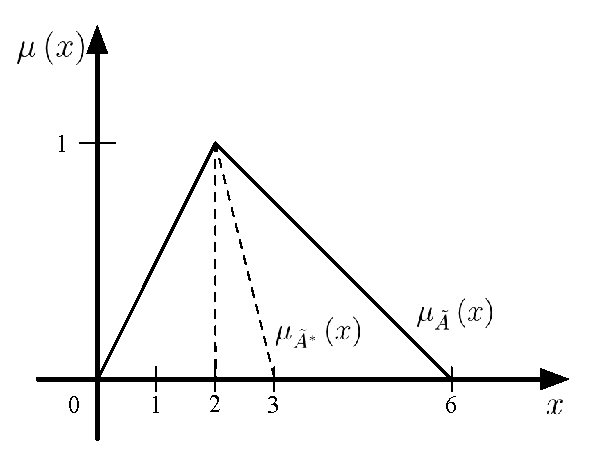
\includegraphics[width=0.7\textwidth]{sample-224}
    \caption{Исходное нечёткое число и~его модификация при~выборе средней точки $\alpha$-интервала}
    \label{fig:sample-224}
  }
\end{figure}

Очевидно, что на~вид модифицированных чисел (и,~соответственно, на~итоговый результат решения задачи) влияние будут оказывать как характеристики самих нечётких чисел~--- мода, коэффициенты нечёткости,~--- так и~принцип, согласно которому выбирается точка $\overline{x}\left( \alpha  \right)$. В~статье~\cite{Vorontsov_PI} предложено обобщение принципа, вводимого в~\cite{Lebedev}~--- значение $\overline{x}\left( \alpha  \right)$ выбирается с~помощью линейного параметрического преобразования $L$:
\begin{equation}
  \label{eq:L-transform-base}
  \bar{x}\left( \alpha  \right)=L\left( X_\alpha \right)=\lambda x^L \left( \alpha  \right)+\left( 1-\lambda  \right) x^R \left( \alpha  \right).
\end{equation}

Параметр преобразования $\lambda \in \left[ 0;1 \right]$ выбирается индивидуально для каждого числа согласно его характеристикам – величинам коэффициентов нечёткости и длине носителя. Нетрудно убедиться, что мода модифицированного числа $m_{\tilde A^{*}}$ равна
\begin{equation}
\label{eq:L-mode}
  m_{\tilde A^{*}}=\bar{x}\left( 1 \right),
\end{equation}
а ненулевой коэффициент нечёткости и носитель равны по модулю
\begin{equation}
\label{eq:L-support}
  d_{\tilde A^{*}}=\left| \bar{x}\left( 1 \right)-\bar{x}\left( 0 \right) \right|.
\end{equation}

Если известно уравнение~\eqref{eq:L-transform-base}, то, с~учётом~\eqref{eq:L-mode} и~\eqref{eq:L-support}, модифицированное нечёткое число можно представить в виде тройки $\displaystyle \left\langle \bar{x}\left( 1 \right);\left| \bar{x}\left( 1 \right)-\bar{x}\left( 0 \right) \right|;0 \right\rangle$ (число LL-типа) или $\displaystyle \left\langle \bar{x}\left( 1 \right);0;\left| \bar{x}\left( 1 \right)-\bar{x}\left( 0 \right) \right| \right\rangle$ (число RR-типа). Тип модифицированного числа можно определить по коэффициенту при $\alpha$ в~\eqref{eq:L-transform-base}: если он больше нуля, то~число LL-типа, если меньше~--- RR-типа.

Исходя из механизма построения модифицированных нечётких чисел, очевидно, что преобразование~\eqref{eq:L-transform-base} сокращает информативность исходной нечёткой величины. Чтобы выяснить, насколько существенны потери нечёткой информации при различных значениях параметра $\lambda$, проведём исследование свойств преобразования $L$.

Для исследования свойств преобразования $L$ введём следующие характеристические показатели нечёткого числа, которые определяют его информативность с~точки зрения принятия решений~\cite{VSU-1, Alushta-1}, а~также, по~аналогии с~\cite{Spesivtsev}, позволяют производить анализ и~вычисления в~форме, нечувствительной к~знаку нечёткого числа:
\begin{itemize}
  \item длина носителя $d_{\tilde A}$;
  \item мода $m_{\tilde A}$;
  \item степень асимметрии $AS_{\tilde A}$.
\end{itemize}

При использовании записи треугольного числа с помощью коэффициентов нечёткости, длина носителя определяется как их сумма:
\begin{equation}
\label{eq:support-length}
  d_{\tilde A}=a+b
\end{equation}

\begin{mydef}
  Степенью асимметрии $AS_{\tilde A}$ будем называть характеристику треугольного нечёткого числа, определяемую как разность площадей прямоугольных треугольников, на которые исходное нечёткое число делится модой (рис.~\ref{fig:as-degree})~\cite{VSU-1}.
\end{mydef}
\begin{figure}[h!]
  \centering
  {
    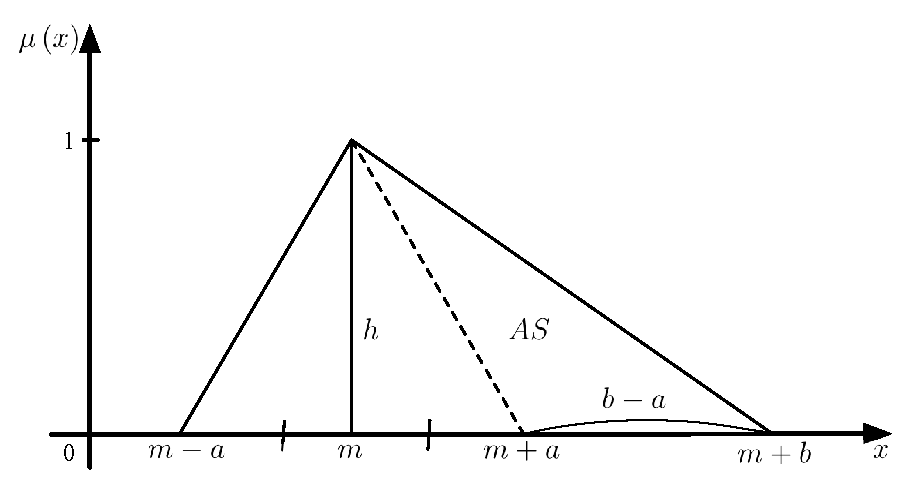
\includegraphics[width=0.8\textwidth]{as-degree}
    \caption{Геометрический смысл степени асимметрии числа}
    \label{fig:as-degree}
  }
\end{figure}

Площадь левого треугольника $\displaystyle S_1=\frac{1}{2}ah(\tilde A)=\frac{a}{2}$, правого $\displaystyle S_2=\frac{1}{2}bh\left(\tilde A \right)=\frac{b}{2}$, отсюда
\begin{equation}
\label{eq:as-param}
  AS_{\tilde A}=S_2-S_1=\frac{b-a}{2}\in \left[ -\frac{a}{2};\frac{b}{2} \right].
\end{equation}

Если $\tilde{A}$ является числом $LL$($RR$)-типа, то $AS_{\tilde A}$, согласно~\eqref{eq:as-param}, принимает значение $\displaystyle -\frac{a}{2}$ ($\displaystyle \frac{b}{2}$).

Очевидно, что~запись треугольного нечёткого числа в~виде тройки $\left(m_{\tilde A}, d_{\tilde A}, AS_{\tilde A} \right)$ эквивалентна введённым ранее способам записи через коэффициенты нечёткости $\left( m;a;b \right)$ и~точки пересечения с~осью $Ox$ $\left( x^L;m;x^R \right)$. При~известных степени асимметрии~$AS_{\tilde A}$ и~длине носителя~$d_{\tilde A}$, коэффициенты нечёткости определяются по~формуле
\begin{equation}
\label{eq:mdas-to-abm}
	\left[ \begin{aligned}
      & a=\frac{d_{\tilde A}-2AS_{\tilde A}}{2} \\ 
      & b=\frac{d_{\tilde A}+2AS_{\tilde A}}{2} \\ 
    \end{aligned} \right.
\end{equation}

Справедливость~\eqref{eq:mdas-to-abm} можно проверить, подставив соответствующие значения для~$AS_{\tilde A}$ и $d_{\tilde A}$ из~формул~\eqref{eq:support-length} и~\eqref{eq:as-param}.

\textbf{Пример.} Найдём эквивалентную форму записи для~треугольного числа $\tilde{A}=\left\langle 5;3;2 \right\rangle $ в~виде тройки <<мода~--- носитель~--- степень~асимметрии>>.

Согласно формуле \eqref{eq:support-length} длина носителя равна
\begin{equation*}
  d_{\tilde A}=a+b=3+2=5
\end{equation*}
Степень асимметрии $AS_{\tilde A}$ вычисляется по формуле~\eqref{eq:as-param}
\begin{equation*}
  AS_{\tilde A}=\frac{2-3}{2}=-0,5
\end{equation*}
Таким образом, число $\tilde{A}$ представляется в виде тройки $\left( 5;5;-0,5 \right)$.

\subsection{Свойства преобразования $L$}

\begin{prop}
\label{prop:L-prop1}
Преобразование $L$ сохраняет моду нечёткого числа. Другими словами, $\forall \lambda (\alpha ):\ m_{\tilde A}=m_{\tilde A^{*}}$.
\end{prop}
\textbf{Доказательство.} Перепишем свойство с~учётом равенств:
\begin{gather*}
  x^L(\alpha )=x_{A}^{L}+\alpha (m_A-x_{A}^{L}); \\ 
  x^R(\alpha )=x_{A}^{R}+\alpha (m_A-x_{A}^{R}).
\end{gather*}

При~$\alpha=1$ 
\begin{gather*}
  x^L(1)=x_{\tilde A}^{L}+1\left( m_{\tilde A}-x_{\tilde A}^{L} \right)=m_{\tilde A}; \\ 
  x^R(1)=x_{\tilde A}^{R}+1\left( m_{\tilde A}-x_{\tilde A}^{R} \right)=m_{\tilde A},
\end{gather*}
поэтому при подстановке $\alpha=1$ в~преобразование~\eqref{eq:L-transform-base} получаем:
\begin{equation}
\label{eq:L-prop1-proof}
  \bar{x}\left( 1 \right)=\lambda x^L\left( 1 \right)+\left( 1-\lambda  \right)x^R\left( 1 \right)=\lambda m_{\tilde A}+\left( 1-\lambda \right)m_{\tilde A}=m_{\tilde A}.
\end{equation}
Выражение~\eqref{eq:L-prop1-proof} доказывает, что моды модифицированного и исходного чисел совпадают при любых значения параметров преобразования~\eqref{eq:L-transform-base}.

\begin{prop}
\label{prop:L-prop2}
При некоторых значениях параметра $\lambda$ преобразование $L$ сохраняет
\begin{enumerate}
  \item знак степени асимметрии, т.е. $\exists \lambda \in [0;1]:\ sign(AS_{\tilde A})=sign(AS_{\tilde A^{*}})$;
  \item значение степени асимметрии, т.е. $\exists \lambda \in [0;1]:\ AS_{\tilde A}=AS_{\tilde A^{*}}$.
\end{enumerate}
\end{prop}
\textbf{Доказательство.} Вначале докажем первое утверждение. Степень асимметрии исходного числа $\tilde A$ определяется выражением~\eqref{eq:as-param}. Модифицированное число имеет только~один ненулевой коэффициент нечёткости, который равен $\left| \bar{x}\left( 1 \right)-\bar{x}\left( 0 \right) \right|$. Кроме того, согласно свойству~\ref{prop:L-prop1}, мода числа при~преобразовании сохраняется. Поэтому абсолютная величина степени асимметрии равна
\begin{equation}
\label{eq:L-prop2-as}
  \left| AS_{\tilde A^{*}} \right|=\frac{\left| m-\bar{x}\left( 0 \right) \right|}{2}.
\end{equation}
Поскольку
\begin{equation}
\label{eq:L-prop2-x0}
  \bar{x}\left( 0 \right)=\lambda {{x}^{L}}\left( 0 \right)+\left( 1-\lambda  \right){{x}^{R}}\left( 0 \right)=m+b-\lambda \left( a+b \right),
\end{equation}
то~выражение~\eqref{eq:L-prop2-as} принимает~вид
\begin{equation}
\label{eq:L-prop2-asab}
  \left| AS_{\tilde A^{*}} \right|=\frac{\left| b-\lambda \left( a+b \right) \right|}{2}.
\end{equation}

Если исходное нечёткое число симметричное, т.\,е. $a=b$, то~степень его~асимметрии равна нулю. В этом случае равенство степеней асимметрии достигается при $\displaystyle \lambda =\frac{1}{2}$ -при подстановке данного значения в~\eqref{eq:L-prop2-asab} имеем верное равенство:
\begin{equation*}
  \left| AS_{\tilde A^{*}} \right|=\frac{\left| b-\lambda \left( a+b \right) \right|}{2}=\frac{1}{2}\left| b-\frac{b+b}{2} \right|=\frac{1}{2}\left| b-b \right|=0.
\end{equation*}

Если $a>b$, то~$AS_{\tilde A}<0$, и~для выполнения первого пункта свойства необходимо, чтобы модифицированное число было числом $LL$-типа. Это достигается при
\begin{equation}
\label{eq:L-prop2-ll-inequality}
  \bar{x}\left( 0 \right)<m.
\end{equation}
Преобразовывая~\eqref{eq:L-prop2-ll-inequality} с~использованием~\eqref{eq:L-prop2-x0}, получаем, что $b-\lambda \left( a+b \right)<0$, и~в~результате 
\begin{equation*}
  \lambda \in \left( \frac{b}{a+b};1 \right].
\end{equation*}

При $a<b$ $AS_{\tilde A}>0$, и~модифицированное число должно быть числом $RR$-типа, т.\,е.
\begin{equation}
\label{eq:L-prop2-rr-inequality}
  \bar{x}\left( 0 \right)>m.
\end{equation}
По~аналогии, подставляя~в~\eqref{eq:L-prop2-rr-inequality} значение $\bar{x}\left( 0 \right)$ из~\eqref{eq:L-prop2-x0}, получаем, что $b-\lambda \left( a+b \right)>0$, и 
\begin{equation*}
  \lambda \in \left[ 0;\frac{b}{a+b} \right).
\end{equation*}

Таким образом, знак степени асимметрии сохраняется при выполнении следующих условий:
\begin{equation*}
  \left[ \begin{aligned}
    & \lambda \in \left[ 0;\frac{b}{a+b} \right);\ a<b \\ 
    & \lambda =0,5;\ a=b \\ 
    & \lambda \in \left( \frac{b}{a+b};1 \right];\ a>b
  \end{aligned} \right.
\end{equation*}

Докажем теперь второе утверждение. Для этого покажем, что уравнение
\begin{equation}
\label{eq:L-prop2-as-equation}
  A{{S}_{{\tilde{A}}}}=A{{S}_{{{{\tilde{A}}}^{*}}}}
\end{equation}
имеет решения при $\lambda \in \left[ 0;1 \right]$. Пусть, для~определённости, у~исходного числа $a>b$, тогда $AS_{\tilde A}<0$, и поэтому должно быть справедливо неравенство $AS_{\tilde A^{*}}<0$. Пользуясь выражением~\eqref{eq:L-prop2-as}, получаем
\begin{equation}
\label{eq:L-prop2-as-abx}
  A{{S}_{{{{\tilde{A}}}^{*}}}}=\frac{\bar{x}\left( 0 \right)-m}{2}=\frac{b-\lambda \left( a+b \right)}{2}<0
\end{equation}
Подставляя~\eqref{eq:as-param} и~\eqref{eq:L-prop2-as-abx} в~\eqref{eq:L-prop2-as-equation}, приходим к уравнению
\begin{equation}
\label{eq:L-prop2-as-proof}
  \frac{b-a}{2}=\frac{b-\lambda \left( a+b \right)}{2}.
\end{equation}
Его~решением является значение $\displaystyle \lambda =\frac{a}{a+b}=\frac{a}{d}$.

Если же $a<b$, то~$AS_{\tilde A}>0$, и~выражение~\eqref{eq:L-prop2-as-abx} должно быть положительным. В~итоге имеем то же самое уравнение~\eqref{eq:L-prop2-as-proof}.

Таким образом, при $\displaystyle \lambda =\frac{a}{a+b}$ значение степени асимметрии числа сохраняется.

\begin{prop}
\label{prop:L-prop3}
Модифицированное число всегда содержится внутри исходного числа. Другими словами, 
\begin{equation*}
  \forall \lambda \in \left[ 0;1 \right]: A_{\alpha}^{*}\subset A_\alpha;\ d_{\tilde A} \geqslant d_{\tilde A^{*}},
\end{equation*}
т.\,е. преобразование~$L$ уменьшает длину носителя нечёткого числа и~оставляет $\alpha$-интервалы модифицированного числа в~рамках $\alpha$-интервалов исходного числа.
\end{prop}
\textbf{Доказательство.} Вначале докажем, что $\forall \lambda \in \left[ 0;1 \right]\ d_{\tilde A}\geqslant d_{\tilde A^{*}}$. Решим данное неравенство и~покажем, что отрезок $\left[ 0;1 \right]$ содержится внутри решения. Очевидно, что
\begin{equation*}
  d_{\tilde A^{*}}=\left| \bar{x}\left( 1 \right)-\bar{x}\left( 0 \right) \right|=\left| m_{\tilde A}-\left( m_{\tilde A}-b+\lambda \left( a+b \right) \right) \right|=\left| b-\lambda \left( a+b \right) \right|,
\end{equation*}
и поэтому
\begin{equation*}
  \left| b-\lambda (a+b) \right|\leqslant a+b.
\end{equation*}
Раскрывая модуль, получаем систему неравенств
\begin{equation*}
  \left\{ \begin{aligned}
    & b-\lambda \left( a+b \right)\geqslant -a-b; \\ 
    & b-\lambda \left( a+b \right)\leqslant a+b,
  \end{aligned} \right.
\end{equation*}
Её решением является отрезок $\displaystyle \left[ -\frac{a}{a+b};1+\frac{b}{a+b} \right]$. Ввиду того, что $a,b\geqslant 0$, этот отрезок содержит в себе интервал $\left[ 0;1 \right]$.

Теперь покажем, что $\forall \lambda \in \left[ 0;1 \right]:A_{\alpha}^{*}\subset A_\alpha$. Очевидно, что $\alpha$-интервал модифицированного числа будет ограничен с одной стороны значением моды $m_{\tilde A}$, а с другой~--- значением $\bar{x}\left( \alpha  \right)$. В силу определения нечёткого числа
\begin{equation}
\label{eq:L-prop2-bordercase1}
  \forall \alpha \in \left[ 0;1 \right]\ x_{\tilde A}^{L}(\alpha )\leqslant m_{\tilde A}\le x_{\tilde A}^{R}(\alpha).
\end{equation}
Кроме того, из~определения~\eqref{eq:L-transform-base} преобразования L следует, что
\begin{equation}
\label{eq:L-prop2-bordercase2}
  \forall \alpha \in \left[ 0;1 \right]\ x_{\tilde A}^{L}(\alpha )\leqslant \bar{x}(\alpha )\leqslant x_{\tilde A}^{R}(\alpha).
\end{equation}

Исходя из~\eqref{eq:L-prop2-bordercase1} и~\eqref{eq:L-prop2-bordercase2}, $\left[ x_{\tilde A}^{L}(\alpha );x_{\tilde A}^{R}(\alpha ) \right]\supset \left[ x_{\tilde A}^{M};\bar{x}(\alpha ) \right]$ для LL-числа (соответственно, $\left[ x_{\tilde A}^{L}(\alpha ); x_{\tilde A}^{R}(\alpha ) \right] \supset \left[ \bar{x}(\alpha ); x_{\tilde A}^{M} \right]$ для RR-числа).

Проиллюстрируем доказанные выше свойства примером. Пусть $\tilde{A}=\left\langle 4;5;1 \right\rangle $. Степень его асимметрии равна
\begin{equation*}
  AS_{\tilde A}=\frac{1-5}{2}=-2,
\end{equation*}
а~длина носителя $d_{\tilde A}$
\begin{equation*}
  d_{\tilde A}=5+1=6.
\end{equation*}
Уравнения для левой и правой ветвей функции принадлежности принимают вид
\begin{equation}
\label{eq:L-propsample-lrmembership}
  \left[ \begin{aligned}
    & {{x}^{L}}\left( \alpha  \right)=-1+5\alpha; \\ 
    & {{x}^{R}}\left( \alpha  \right)=5-\alpha.
  \end{aligned} \right.
\end{equation}

Выполним преобразование $L$ с параметром $\lambda =\frac{1}{4}$ с~учётом~\eqref{eq:L-propsample-lrmembership}:
\begin{equation}
\label{eq:L-propsample-xmid}
  \bar{x}\left( \alpha  \right)=\frac{1}{4}\left( 5\alpha -1 \right)+\frac{3}{4}\left( 5-\alpha  \right)=\frac{1}{4}\left( 5\alpha -1+15-3\alpha  \right)=\frac{1}{4}\left( 14+2\alpha  \right)=3,5+0,5\alpha.
\end{equation}

Поскольку коэффициент при~$\alpha $ в~выражении~\eqref{eq:L-propsample-xmid} больше нуля, то~число $\tilde A^{*}$ является числом LL-типа. Мода числа $\tilde A^{*}$, согласно свойству~\ref{prop:L-prop1}, равна 4, а~левый коэффициент нечёткости равен длине носителя и~равен
\begin{equation*}
  a=d_{\tilde A^{*}}=\left| \bar{x}\left( 1 \right)-\bar{x}\left( 0 \right) \right|=\left| 4-\left( 3,5-0,5\cdot 0 \right) \right|=0,5.
\end{equation*}

Таким образом, число $\tilde A^{*}$ может быть записано в виде тройки $\left\langle 4;0,5;0 \right\rangle $. Степень его асимметрии, согласно свойству~\ref{prop:L-prop2}, сохраняет знак относительно $AS_{\tilde A}$ и равна
\begin{equation*}
  AS_{\tilde A^{*}}=\frac{0-0,5}{2}=-0,25.
\end{equation*}

Исходное и~модифицированное числа изображены на~рис.~\ref{fig:l-transform-properties-sample}. На~нём наглядно иллюстрируется свойство~\ref{prop:L-prop3}~--- модифицированное число $\tilde A^{*}$ целиком расположено внутри границ исходного числа.
\begin{figure}[h!]
  \centering
  {
    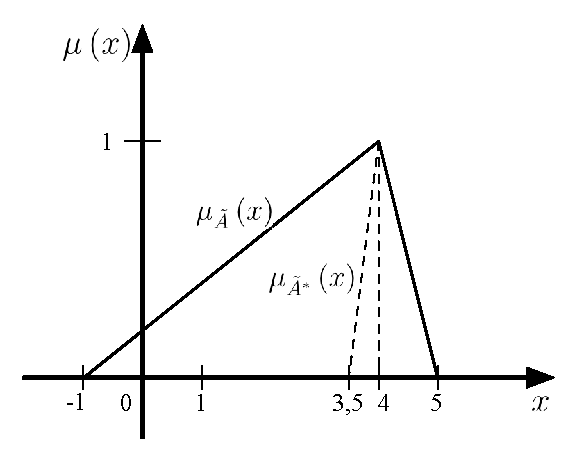
\includegraphics[width=0.65\textwidth]{l-transform-properties-sample}
    \caption{Иллюстрация свойств преобразования L}
    \label{fig:l-transform-properties-sample}
  }
\end{figure}

Из~доказанных выше свойств следует, что~применение преобразования~$L$ к~нечетким исходным данным в~основном сохраняет их~информативность при~целенаправленном выборе параметра преобразования~\cite{VSU-1}. Уменьшение длины носителя при~определенных оговорках можно рассматривать как~положительное явление, поскольку при~этом повышается общая устойчивость решения~\cite{Vorontsov_PI}.

Рассмотрим следствия из~доказанных ранее свойств преобразования~$L$ и~рекомендации по~выбору параметра $\lambda$.
\begin{cor}
Модифицированное нечёткое число, получаемое с помощью преобразования L с~$\lambda =0,5$ из симметричного нечёткого числа $\left\langle m;a;a \right\rangle$, является нечётким синглтоном.
\end{cor}
Действительно, при указанном значении $\lambda $, используя выражения, получаем:
\begin{equation*}
  \bar{x}\left( \alpha  \right)=\frac{1}{2}\left( m-a+a\alpha  \right)+\frac{1}{2}\left( m+b-b\alpha  \right)=\frac{1}{2}\left( m-a+a\alpha +m+a-a\alpha  \right)=m.
\end{equation*}
Это следствие накладывает ограничения на возможность использования симметричных нечётких чисел в задачах, поскольку все нечёткие вычисления с~использованием преобразования~$L$ в этом случае будут сведены к обычным алгебраическим операциям над модами чисел~\cite{Alushta-1, VSU-1}.

\begin{cor}
Применение преобразования~$L$ с~параметром $\displaystyle \lambda =\frac{a}{a+b}$ к~числу LL/RR-типа не изменяет данного числа.
\end{cor}
В~самом деле, для LL-числа $b=0$, поэтому $x_{{\tilde{A}}}^{R}\left( \alpha  \right)=m+b-b\alpha=m$, $\lambda=\frac{a}{a+0}=1$. Отсюда
\begin{equation*}
  \bar{x}\left( \alpha  \right)=\lambda \left( m-a+a\alpha  \right)+\left( 1-\lambda  \right)m=m-a+a\alpha =x_{\tilde A}^{L}\left( \alpha  \right).
\end{equation*}
Для RR-числа $a=0$, отсюда $x_{\tilde A}^{L}\left( \alpha  \right)=m-a+a\alpha=m$ и $\lambda =\frac{0}{b+0}=0$. Ввиду этого
\begin{equation*}
  \bar{x}\left( \alpha  \right)=\lambda m+\left( 1-\lambda  \right)\left( m+b-b\alpha  \right)=m+b-b\alpha =x_{\tilde A}^{R}\left( \alpha  \right).
\end{equation*}

Отдельно выделим несколько наиболее интересных значений $\lambda$.

1. $\displaystyle \lambda =\frac{a}{a+b}=\frac{a}{d_{\tilde A}}$. Как уже было показано выше, при данном значении сохраняется значение степени асимметрии~\cite{VSU-1}.

Проиллюстрируем это на следующем примере. Пусть $\tilde{A}=\left\langle 1;4;6 \right\rangle $. Значение $\displaystyle \lambda =\frac{4}{4+6}=\frac{2}{5}$, степень асимметрии $\displaystyle AS_{\tilde A}=\frac{6-4}{2}=1$, а уравнения правой и левой ветвей
\begin{equation*}
  \left[ \begin{aligned}
    & {{x}^{L}}\left( \alpha  \right)=-3+4\alpha; \\ 
    & {{x}^{R}}\left( \alpha  \right)=7-6\alpha. \\ 
  \end{aligned} \right.
\end{equation*}

Преобразование L даёт следующий результат:
\begin{equation*}
  \bar{x}\left( \alpha  \right)=\frac{2}{5}\left( -3+4\alpha  \right)+\frac{3}{5}\left( 7-6\alpha  \right)=\frac{1}{5}\left( -6+8\alpha +21-18\alpha  \right)=3-2\alpha.
\end{equation*}

Полученное в результате преобразования число $\tilde A^{*}$ является числом RR-типа, поэтому степень его~асимметрии положительна и, согласно~\eqref{eq:L-prop2-as}, равна
\begin{equation*}
  AS_{\tilde A^{*}}=\frac{\left| 1-\left( 3-2\cdot 0 \right) \right|}{2}=1.
\end{equation*}

2. $\displaystyle \lambda =\frac{b}{a+b}=\frac{b}{d_{\tilde A}}$. Преобразование~$L$ с~таким значение параметра уничтожает нечёткую информацию, заложенную экспертом в число~\cite{Vorontsov_PI}, поскольку в~этом случае модифицированное число превращается в~чёткое:
\begin{gather*}
  \bar{x}\left( \alpha  \right)=\frac{b}{a+b}\left( m-a+a\alpha \right)+\left( 1-\frac{b}{a+b} \right)\left( m+b-b\alpha \right)={}\\
  {}=\frac{b\left( m-a+a\alpha  \right)+a\left( m+b-b\alpha \right)}{a+b}={} \\ 
  {}=\frac{bm-ab+ab\alpha +am+ab-ab\alpha }{a+b}=\frac{am+bm}{a+b}=m. 
\end{gather*}

3. При $\displaystyle \lambda =\frac{b}{d_{\tilde A}}-\frac{b-a}{3\left( b+a \right)}=\frac{2b+a}{3\left( b+a \right)}=\frac{2b+a}{3d_{\tilde A}}$ значение $\bar{x}(\alpha )$ является проекцией центра тяжести треугольника, построенного на отрезке $\left[ {{x}^{L}}(\alpha ), x^R\left(\alpha \right) \right]$ как на~основании, на~ось~$Ox$ (см.~рис.~\ref{fig:l-midpoint}).
\begin{figure}[h!]
  \centering
  {
    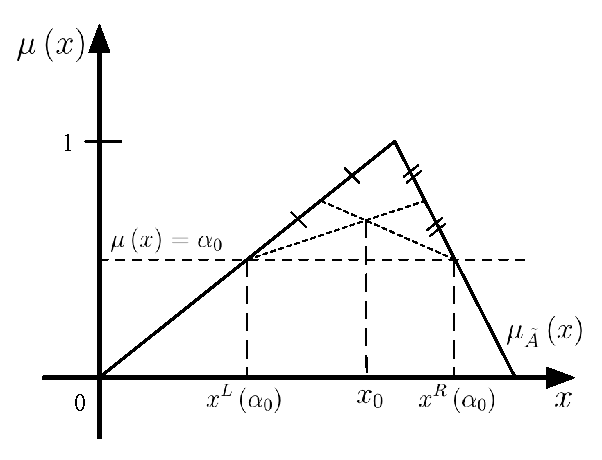
\includegraphics[width=0.7\textwidth]{l-midpoint}
    \caption{Поиск проекции центра тяжести $\alpha$-сечения}
    \label{fig:l-midpoint}
  }
\end{figure}

Данное значение получается следующим образом. Координата $x_0 \left( \alpha  \right)$ центра тяжести $\alpha$-сечения треугольного числа рассчитывается как
\begin{equation}
\label{eq:x-weightcentre}
  x_0\left( \alpha  \right)=\frac{x^L\left( \alpha  \right)+m+x^R\left( \alpha  \right)}{3}.
\end{equation}

Значения $x^L\left( \alpha  \right)$ и $x^R\left( \alpha \right)$ равны
\begin{equation}
\label{eq:xlxr-weightcentre}
  \left[ \begin{aligned}
    & x^L\left( \alpha  \right)=m-a+a\alpha; \\ 
    & x^R\left( \alpha  \right)=m+b-b\alpha.
  \end{aligned} \right.
\end{equation}

Из~\eqref{eq:x-weightcentre} и~\eqref{eq:xlxr-weightcentre} следует, что
\begin{gather}
  x_0\left( \alpha  \right)=\frac{x^L\left( \alpha  \right)+m+x^R\left( \alpha  \right)}{3}=\frac{m-a+a\alpha +m+m+b-b\alpha }{3}={} \notag \\ 
  \label{eq:x0-calculated1}
  {}=\frac{3m-\left( a-b \right)+\alpha \left( a-b \right)}{3}=m+\frac{\left( a-b \right)\left( \alpha -1 \right)}{3}.
\end{gather}

Преобразование $L$ вычисляется по формуле
\begin{gather}
  \bar{x}\left( \alpha  \right)=\lambda x^L\left( \alpha  \right)+\left( 1-\lambda  \right)x^R\left( \alpha  \right)=\lambda \left( m-a+a\alpha  \right)+\left( 1-\lambda  \right)\left( m+b-b\alpha  \right)={} \notag \\ 
  {}=\lambda \left( m-a+a\alpha -m-b+b\alpha  \right)+b\left( 1-\alpha  \right)+m={} \notag \\
  \label{eq:x0-calculated2}
  {}=\lambda \left( a+b \right)\left( \alpha -1 \right)+b\left( 1-\alpha  \right)+m.
\end{gather}

Приравнивая результаты~\eqref{eq:x0-calculated1} и~\eqref{eq:x0-calculated2}, получаем:
\begin{gather*}
  m+\frac{\left( a-b \right)\left( \alpha -1 \right)}{3}=m+b\left( 1-\alpha  \right)+\lambda \left( a+b \right)\left( \alpha -1 \right); \\
  \left( a-b \right)\left( \alpha -1 \right)=-3b\left( \alpha -1 \right)+3\lambda \left( a+b \right)\left( \alpha -1 \right).  
\end{gather*}
 
При~$\alpha=1$ равенство выполняется для~всех $\lambda \in \left[ 0; 1\right]$. Для остальных $\alpha$, поделим обе части равенства на~$\alpha-1$:
\begin{equation*}
  a-b=-3b+3\lambda \left( a+b \right),
\end{equation*}
откуда получается искомое значение $\lambda$~\cite{VSU-1}.